\chapter{Fundamento teórico}\label{chap:teo}
En este capítulo se presentan los conceptos y términos fundamentales que se
utilizan en el proyecto, para proporcionar una base teórica sobre la que se
desarrolla el trabajo. Se discuten los conceptos de \textit{data lake},
\textit{procesos ETL} y \textit{dashboards}, que son fundamentales para el
desarrollo del proyecto.

\section{\textit{Big data}}\label{sec:bigdata}
El término \textit{big data} se refiere a la gestión y análisis de grandes
volúmenes de datos que no pueden ser tratados de manera convencional. Estos
datos se caracterizan por su volumen, velocidad y variedad, lo que hace que sea
difícil procesarlos con las herramientas tradicionales de gestión de datos.

El \textit{big data} se caracteriza por tres características principales:
volumen, variedad y velocidad. Estas características se conocen como las
``tres V'' del \textit{big data}:

\begin{itemize}
	\item \textbf{Volumen:} se refiere a la cantidad de datos que se generan y
		almacenan en un determinado periodo de tiempo. El volumen de datos que
		se maneja en el \textit{big data} es mucho mayor que el que se maneja en
		los sistemas tradicionales de gestión de datos.
	\item \textbf{Variedad:} se refiere a la diversidad de fuentes y formatos de
		los datos que se manejan en el \textit{big data}. Los datos pueden
		provenir de diferentes fuentes, como bases de datos, archivos de
		registros y APIs, y pueden estar en diferentes formatos, como texto,
		imágenes, audio, vídeo, etc.
	\item \textbf{Velocidad:} se refiere a la velocidad a la que se generan y se
		procesan los datos. En este ámbito, los datos se generan y se procesan a
		una velocidad mucho mayor que en los sistemas tradicionales de gestión
		de datos.
\end{itemize}

El \textit{big data} es un fenómeno que ha surgido en los últimos años debido al
crecimiento exponencial de los datos que se generan y almacenan en todo el
mundo. Este crecimiento ha sido impulsado por el aumento de la conectividad y el
uso de dispositivos móviles, que han permitido a las empresas y a los usuarios
generar y almacenar grandes cantidades de datos en todo el mundo.

\section{Paradigmas de almacenamiento de datos}\label{sec:paradigmas}
En el ámbito del \textit{big data}, existen diferentes paradigmas de
almacenamiento de datos que se utilizan para almacenar y analizar grandes
cantidades de información. Los tres paradigmas a considerar para este proyecto
son los \textit{data warehouses}, los \textit{data lakes} y los
\textit{data lakehouses}.

\subsection{Data warehouse}\label{sec:warehouse}
Un \textit{data warehouse}\footnote{
	\url{https://aws.amazon.com/es/data-warehouse/}
}, también conocido en español como almacén de datos, es una base de datos que
se utiliza para almacenar y analizar grandes cantidades de datos de manera
eficiente. Los almacenes de datos proporcionan acceso rápido y compatible con
plataformas de consultas (como SQL) a grandes cantidades de datos, lo que
permite a los analistas y a los científicos de datos realizar análisis complejos
sobre los datos almacenados.

Todos los datos almacenados en un \textit{data warehouse} se encuentran en un
formato común, para lo que se aplican procesos ETL (extracción, transformación y
carga) que transforman los datos de diferentes fuentes en un formato común. Esto
significa que la información se encuentra en un formato o esquema optimizado y
específico, lo que facilita su manipulación y análisis pero limita la
flexibilidad al acceso de los datos y genera costes adicionales en el caso de
tener que modificar o transferir los mismos para su uso.


\subsection{Data lake}\label{sec:lake}
Los \textit{data lakes}\footnote{
	\url{https://aws.amazon.com/es/what-is/data-lake/}
} son almacenes de datos que guardan grandes cantidades de datos de manera no
estructurada~\cite{mier2023dashboards}. En el ámbito de una empresa, un
\textit{data lake} contiene datos de diferentes fuentes de valor no considerado
hasta su análisis, de manera que su explotación posterior y su análisis no
depende de una estructuración y transformación compleja, reduciendo los costes
de los procesos ETL derivados, una flujo de tareas que se aplican sobre la
información para ingestarla. Esto no quiere decir que no se apliquen estos
procesos a los datos, sino que se aplican de manera más flexible y básica que en
otras estructuras de almacenamiento de datos con esquemas predefinidos, como los
\textit{data warehouses}.~\cite{pwint2018data}

A diferencia de los \textit{data warehouses}, los \textit{data lakes} no tienen
un esquema definido, lo que permite almacenar datos \textit{heterogéneos}. Esto
permite almacenar grandes cantidades de información sin tener que definir un
esquema de antemano, lo que puede ser útil en aquellos casos en los que no se
conoce la estructura de los datos que se van a almacenar.

Estas características de los \textit{data lakes} hacen que sean más atractivos
en el sector empresarial de cara al análisis de información, en contraste con
las estructuras planteadas normalmente en el campo de la investigación
académica.

Para consultar esta gran cantidad de datos almacenados, se suelen utilizar
técnicas de visualización de datos, como los \textit{dashboards}, herramientas
de visualización que permiten observar los datos de manera sencilla y eficiente.

\subsection{Data lakehouse}\label{sec:lakehouse}
Los \textit{data lakehouses} son una combinación funcional de los dos paradigmas
vistos anteriormente, los \textit{data lakes} y los \textit{data warehouses}.
Los \textit{data lakehouses} permiten almacenar datos tanto de manera
estructurada como no estructurada, lo que facilita aprovechar la información al
contar con una única estructura de bajo coste que ofrece a los usuarios que lo
necesiten explorar y analizar los datos según sus necesidades.

\newpage{}
\section{Procesos ETL}\label{sec:etl}
Si anteriormente se presentaban los distintos paradigmas de almacenamiento de
datos, para su creación y mantenimiento se requieren aplicar unos ciertos
procesos que permitan la correcta ingesta y almacenamiento de los datos. Estos
procesos se conocen como \textit{procesos ETL}.

Formalmente se definen los procesos ETL~\cite{mier2023dashboards} como procesos
que combinan datos de múltiples fuentes en un único destino, transformando los
datos en un formato común. Estos procesos se utilizan para extraer datos de
diferentes fuentes, transformarlos en un formato común y cargarlos en un destino
común, como puede ser un \textit{data lake}.

Los procesos ETL, fundamentales en el ámbito de la gestión de datos, presentan
atributos distintivos que facilitan la integración eficaz de información
procedente de diversas fuentes:

\begin{itemize}
	\item \textbf{Adaptabilidad:} los procesos ETL deben de adaptarse a la
		estructura de los datos de la fuente de origen, ya que dichas fuentes
		pueden tener diferentes estructuras y tener tipos de datos diferentes
		(la característica de \textit{heterogeneidad} de los datos que ya se ha
		mencionado).
	\item \textbf{Escalabilidad:} otra de las características clave de los
		procesos ETL es que sean escalables, ya que los datos que se muestran en
		los dashboards suelen ser datos que se generan de manera continua, y por
		lo tanto los procesos ETL deben ser capaces de procesar grandes
		cantidades de datos de manera eficiente. En ocasiones, los procesos ETL
		se pueden realizar en \textit{streaming}, lo que significa que los datos
		se procesan en tiempo real a medida que se generan.
	\item \textbf{Eficiencia:} los procesos ETL deben ser eficientes, puesto que
		el tiempo de procesamiento de los datos es un factor vital en el ámbito
		del \textit{big data}. Los procesos ETL deben ser capaces de procesar
		grandes cantidades de datos en un tiempo razonable para que los datos
		estén disponibles en el menor tiempo posible.
	\item \textbf{Fiabilidad:} la fiabilidad es un componente crítico de todo el
		flujo de datos, ya que estos se utilizan para la toma de decisiones
		importantes de cualquier empresa. Los procesos ETL deben ser capaces de
		procesar los datos de manera fiable y consistente, para que los datos
		que se visualicen y analicen posteriormente sean correctos y fiables.
\end{itemize}

\newpage{}
\subsection{Funcionamiento}
Los procesos ETL se dividen en tres fases principales: \textit{(1) Extraer},
\textit{(2) Transformar} y \textit{(3) Cargar}, como se muestra en el siguiente
diagrama:

\begin{minipage}{\linewidth}
	\centering
	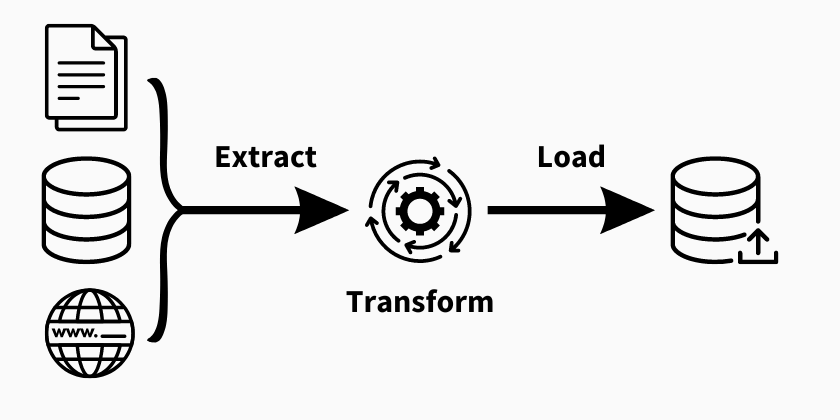
\includegraphics[width=0.8\textwidth]{etl.png}
	\captionof{figure}{Fases de un proceso ETL}
\end{minipage}

Como entrada, se tienen datos presuntamente heterogéneos que no se pueden
analizar de manera eficiente. Tras aplicar todos los pasos de las fases
anteriores, se obtiene como salida un conjunto de datos corregidos y listos para
ser analizados en el destino indicado (en el caso de este proyecto, un
\emph{data lake}).

\paragraph{Extracción (1)}
En este proceso se obtienen los datos de las fuentes de datos, que pueden ser
bases de datos, logs, APIs, etc. En esta fase, se pueden aplicar filtros para
extraer solo los datos que se necesiten, y se pueden extraer datos de múltiples
fuentes \emph{heterogéneas}.

La fase de extracción se puede realizar de dos formas: continua o incremental.
Una extracción incremental se realiza de manera periódica, por ejemplo, cada
hora, cada día o cada semana, y se extraen los datos que se han generado desde
la última extracción. Esto es útil cuando los datos se generan de manera
periódica y se necesita mantener actualizada la información. Por otro lado, en
una extracción continua se extraen los datos en tiempo real según se van
generando. Esto puede ser útil para procesar datos que se generan en tiempo
real, como logs o datos de sensores.

\newpage{}
\paragraph{Transformación (2)}
Durante esta fase, se transforman los datos extraídos en la fase anterior,
normalmente aplicándoles un proceso de limpieza y transformación a un
formato común. En este paso, se pueden aplicar diferentes operaciones a los
datos, como la limpieza, la agregación, la normalización, la conversión de
formatos, etc.

Uno de los tipos de transformaciones de datos más comunes es la limpieza, que
consiste en la revisión y corrección de los datos extraídos, para asegurar que
se almacena información correcta y consistente. Durante esta fase se contemplan
operaciones más complejas, como pueden ser la agregación de datos, la conversión
de formatos, la normalización de datos, el cifrado, etc. La limpieza de datos
puede ser una tarea muy sencilla, como la eliminación de caracteres
delimitadores, o muy compleja, como la corrección de errores en los datos o la
detección de duplicados.

Estos procesos de transformación son vitales cuando el sistema maneja una gran
cantidad de datos heterogéneos de múltiples fuentes de manera simultánea, como
puede ser el caso de un \textit{data lake} o un \textit{data
warehouse}. En el caso del primero, no es necesaria la transformación de los
datos a un formato común, pero si otros procesos clave como la limpieza y la
normalización de los datos, entre otros.

\paragraph{Carga (3)}
En este proceso se vuelcan los datos transformados en el destino final.
Frecuentemente, los datos se almacenan, dependiendo del paradigma de
almacenamiento elegido, en una \textit{data lake}, \textit{data warehouse} o
\textit{data lakehouse} para su posterior análisis.

\newpage{}
\subsection{Alternativas}
Aunque lo más común es el flujo anteriormente explicado de \textit{extracción},
\textit{transformación} y \textit{carga}, existen algunos flujos y procesos
alternativos que evitan algunos de estos pasos, normalmente en casos específicos
que se beneficien del cambio:

\begin{itemize}
	\item \textbf{Virtualización de datos:} capa virtual de abstracción que
		permite acceder a los datos de las fuentes sin necesidad de extraerlos.
		Esto permite ahorrar espacio de almacenamiento y tiempo de
		procesamiento, pero suele ser menos eficiente en términos de rendimiento
		y no es compatible con todas las arquitecturas de datos.

		\begin{minipage}{\linewidth}
			\centering
			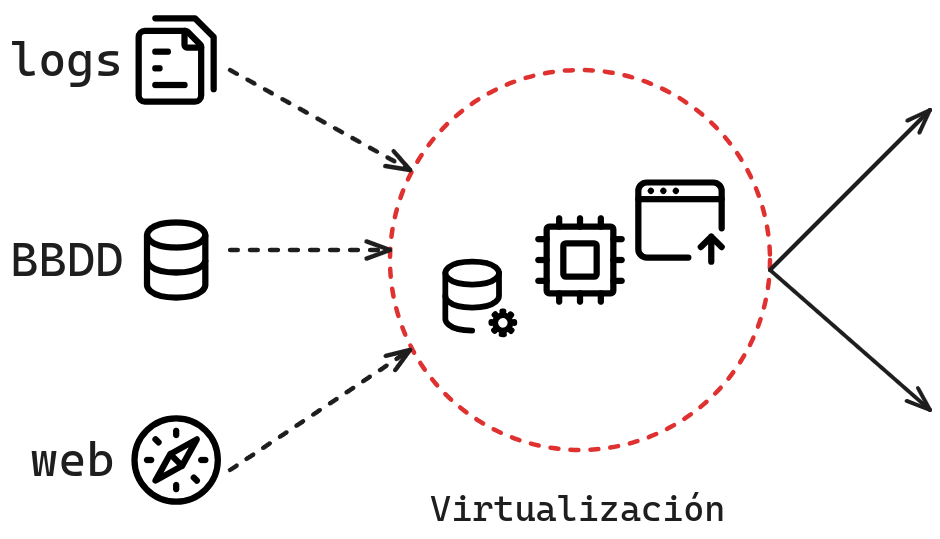
\includegraphics[width=0.65\textwidth]{virt.png}
			\captionof{figure}{Ejemplo de flujo con virtualización}
		\end{minipage}
	\item \textbf{Proceso \textit{ELT}\footnote{\url{https://www.ibm.com/topics/elt}}:}
		en lugar de transformar los datos antes de cargarlos en el destino, se
		cargan los datos en bruto y se transforman en el destino. Funciona bien
		para grandes conjuntos de datos sin estructura que requieran una carga
		(o recarga) contínua, aunque, al igual que la virtualización, puede ser
		menos eficiente o incompatible con algunas arquitecturas de datos, como
		los \textit{data warehouses}.

		\begin{minipage}{\linewidth}
			\centering
			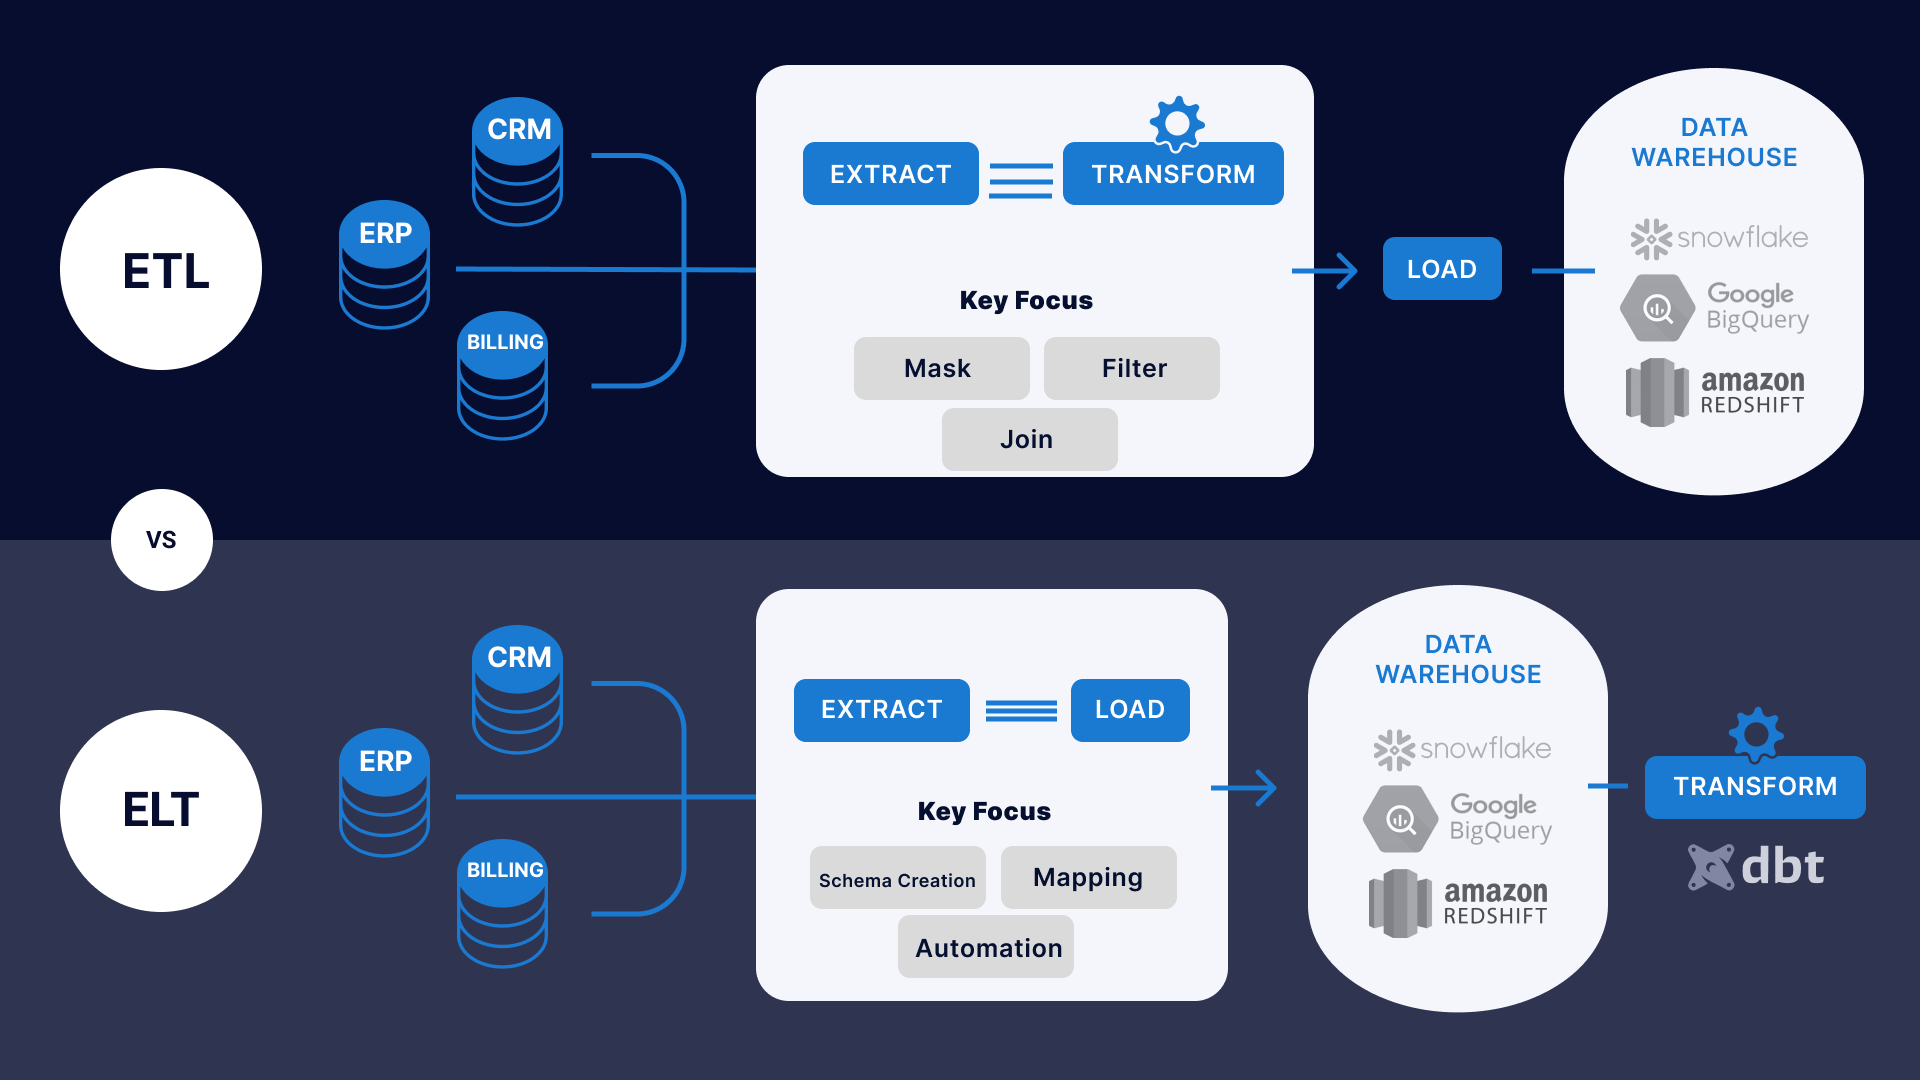
\includegraphics[width=0.75\textwidth]{elt.png}
			\captionof{figure}{Diagrama de flujo de un proceso \textit{ELT}}
		\end{minipage}
\end{itemize}


\newpage{}
\section{Cuadros de mandos (\textit{dashboards})}\label{sec:dashboards}
\paragraph{Definición}
Los cuadros de mandos, en adelante \textit{dashboards},
es un término que se utiliza para referirse a cualquier interfaz gráfica que
muestre información relevante de manera visual sobre un proceso o negocio.
Aunque el término se utiliza en muchos ámbitos: indicadores comerciales, de
producción, de marketing, de calidad, de recursos humanos\ldots, en este
proyecto se utilizará en el ámbito de la monitorización de sistemas y procesos
de negocio.

En el ámbito de deste proyecto, los dashboards reflejan en tiempo real el
rendimiento de actividades o procesos de negocio, y se utilizan para tomar
decisiones informadas basándose en los mismos. Por ejemplo, el dashboard de una
empresa digital puede mostrar desde el rendimiento de la arquitectura en tiempo
real hasta el número de ventas conseguidas, y permitir a los directivos tomar
decisiones informadas sobre el futuro de la empresa (e.g. necesidad de aumentar
la capacidad de los servidores, lanzar una campaña de marketing, etc.).

\paragraph{Características}
Los dashboards cuentan con una serie de características que los hacen útiles
para la toma de decisiones:~\cite{mier2023dashboards}

\begin{itemize}
	\item \textbf{Visualización de datos:} es la característica fundamental de
		cualquier dashboard, y aquella que determina su utilidad.
		La visualización de datos es la ciencia de presentar los datos de manera
		que se pueda extraer información útil y realizar decisiones informadas
		sobre ellos. Un buen dashboard cuenta con gráficas, tablas, indicadores,
		etc. que permiten al usuario entender la información que se está
		presentando con un conocimiento técnico mínimo.
	\item \textbf{Interactividad y personalización:} un dashboard debe permitir
		al usuario interactuar con los datos (filtrarlos, ordenarlos,
		profundizar en ellos...) y ajustar la información que se muestra sobre
		cada proceso o negocio que se esté evaluando (granularidad de la
		información). Esta capacidad asegura que el dashboard se adapte tanto a
		las necesidades actuales como a las evoluciones futuras de lo que se
		esté analizando.
	\item \textbf{Accesibilidad y portabilidad:} un dashboard debe ser accesible
		desde una variedad de situaciones y dispositivos, manteniendo su
		funcionalidad y forma. Aunque normalmente los dashboards se analizan en
		pantallas grandes, es importante que también se puedan consultar en
		otras circunstancias, como dispositivos móviles.
\end{itemize}


\newpage{}
\paragraph{Dashboards planteados}
Para el sistema que se describe, se plantean dos tipos de dashboards diferentes:

\begin{itemize}
	\item \textbf{Dashboards internos}: que reflejan el rendimiento de la
		plataforma en tiempo real. Estos dashboards están destinados al uso
		interno de la empresa, y permiten a los empleados monitorizar el
		rendimiento de la plataforma y tomar decisiones informadas sobre su
		mantenimiento y evolución.
	\item \textbf{Dashboards externos}: que reflejan el rendimiento de las
		ventas y permiten a los clientes tomar decisiones informadas sobre su
		negocio. Estos dashboards están enfocados a los clientes de la empresa,
		y permite a los mismos obtener información relevante sobre su negocio
		que tenga Okticket.
\end{itemize}


\section{Infraestructura como código}
La infraestructura como código (o \textit{IaaS} por sus siglas en inglés) es una
práctica que consiste en gestionar la infraestructura de un sistema de manera
automática y programática mediante código, en lugar de configuraciones manuales.
La infraestructura como código permite gestionar la arquitectura global de un
sistema de manera eficiente y escalable, y facilita la creación y el mantenimiento
de entornos de desarrollo y producción.

En el ámbito de este proyecto, la infraestructura como código se utiliza para
gestionar el despliegue y orquestación de los servicios requeridos para el
\textit{data lake}, como los servicios de ingesta o de visualización de datos.

La infraestructura como código es la parte más importante del desarrollo de este
proyecto, ya que una buena configuración y toma de decisiones a la hora de
desplegar un proyecto de este calibre es vital para el correcto funcionamiento
posterior a la hora de ingestar y tratar con datos heterogéneos.
